% !Mode:: "TeX:UTF-8"

\chapter{}
\textbf{
Suppose that instead of selecting the first activity to finish, we instead select the last activity to start that is compatible with all previously selected activities. Describe how this approach is a greedy algorithm, and prove that it yields an optimal solution.
}

\hspace*{\fill} \\
The algorithm is sorted the activities by the finish time in descent. Then choose activities from the beginning successively guaranteeing that the latter chosen activities is compatible with all previously selected activities.

\begin{figure}[!htbp]
\centering
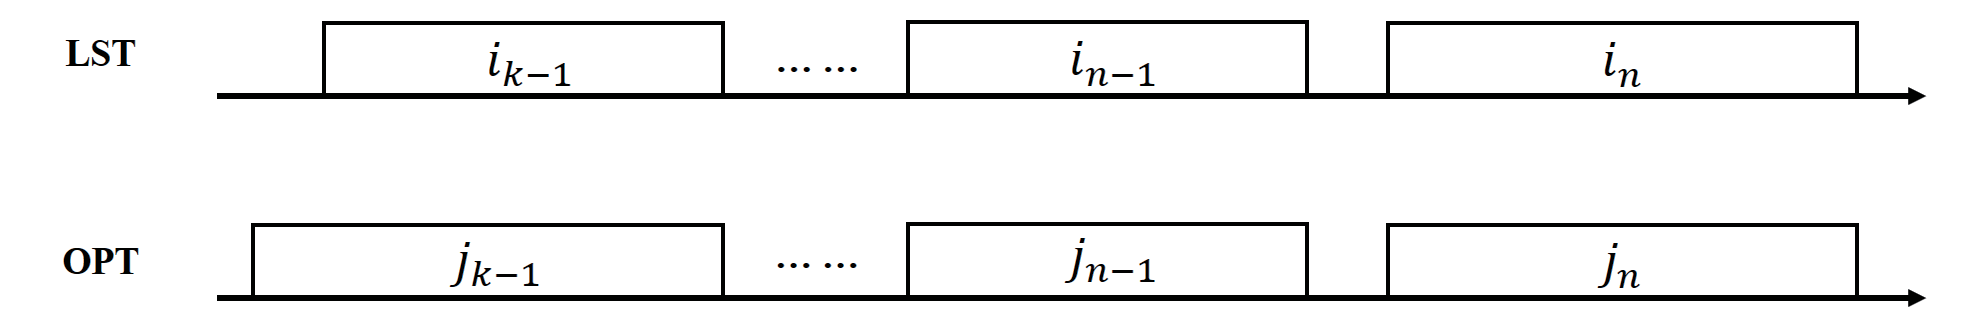
\includegraphics[width=1\textwidth]{figures/1.eps}
\caption{A way of Optimal choice Vs the way of last activity to start}\label{fig_1_1}
\end{figure}
\noindent
\textbf{Proof:}
Let $i_1, i_2, ..., i_n$ be the way of selecting the last activity to start(\emph{LST}). Let $j_1, j_2, ..., j_n$ be the optimal way(\emph{OPT}). We bring each activity into alignment by finished time. Suppose that the most and last $n-k+1$ activities are the same as between $LST$ and $OPT$. As shown in Fig~\ref{fig_1_1}, we can set that the $(k-1)$-th activity is the first different activities which has different finish time. According to the strategy of greedy algorithm, we can replace $(j-1)$-th activity by another activity $(i-1)$ which is no worse than $(i-1)$-th activity. That contradicts to the suppose (that the most number of the last same activities between \emph{LST} and \emph{OPT} is $n-k+1$). So Selecting the last activity to start that is compatible with all previously selected activities is an optimal solution.


